\chapter{Algoritmos de raíz cuadrada}

\index{raíz cuadrada (complejidad)}

Un \key{algoritmo de raíz cuadrada} es un algoritmo que contiene una raíz
cuadrada en su complejidad temporal. Esto puede verse como un ``logaritmo
barato''; la complejidad $O(\sqrt n)$ es mejor que $O(n)$ pero peor que
$O(\log n)$. En cualquier caso, muchos algoritmos de raíz cuadrada son
rápidos y útiles en la práctica.

Por ejemplo, considera el problema de crear una estructura de datos que
soporte dos operaciones en un arreglo: modificar un elemento en la posición
dada y calcular la suma de elementos en el rango dado. Previamente hemos
resuelto el problema utilizando árboles binarios indexados y árboles de
segmentos, que soportan ambas operaciones en tiempo $O(\log n)$. Sin
embargo, ahora resolveremos el problema de otra manera utilizando una
estructura de raíz cuadrada que nos permite modificar elementos en
$O(1)$ y calcular sumas en $O(\sqrt n)$.

La idea es dividir el arreglo en \emph{bloques} de tamaño $\sqrt n$ tal que
cada bloque contenga la suma de sus elementos. Por ejemplo, un arreglo de
16 elementos se divide en bloques de 4 de la siguiente manera:

\begin{center}
    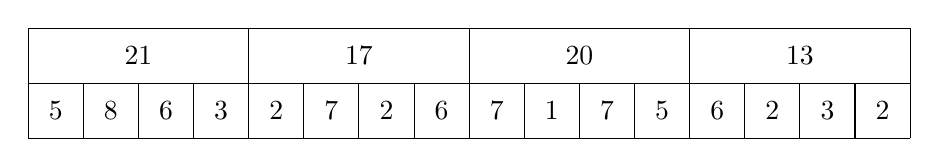
\begin{tikzpicture}[scale=0.7]
        \draw (0,0) grid (16,1);

        \draw (0,1) rectangle (4,2);
        \draw (4,1) rectangle (8,2);
        \draw (8,1) rectangle (12,2);
        \draw (12,1) rectangle (16,2);

        \node at (0.5, 0.5) {5};
        \node at (1.5, 0.5) {8};
        \node at (2.5, 0.5) {6};
        \node at (3.5, 0.5) {3};
        \node at (4.5, 0.5) {2};
        \node at (5.5, 0.5) {7};
        \node at (6.5, 0.5) {2};
        \node at (7.5, 0.5) {6};
        \node at (8.5, 0.5) {7};
        \node at (9.5, 0.5) {1};
        \node at (10.5, 0.5) {7};
        \node at (11.5, 0.5) {5};
        \node at (12.5, 0.5) {6};
        \node at (13.5, 0.5) {2};
        \node at (14.5, 0.5) {3};
        \node at (15.5, 0.5) {2};

        \node at (2, 1.5) {21};
        \node at (6, 1.5) {17};
        \node at (10, 1.5) {20};
        \node at (14, 1.5) {13};

    \end{tikzpicture}
\end{center}

En esta estructura, es fácil modificar los elementos del arreglo, porque
solamente es necesario actualizar la suma de un bloque luego de cada
modificación, que puede hacerse en $O(1)$. Por ejemplo, la siguiente imagen
muestra cómo cambian el valor de un elemento y la suma de su bloque
correspondiente:

\begin{center}
    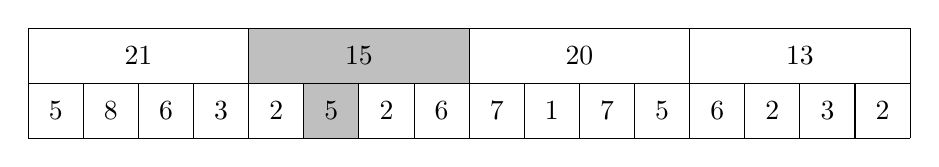
\begin{tikzpicture}[scale=0.7]
        \fill[color=lightgray] (5,0) rectangle (6,1);
        \draw (0,0) grid (16,1);

        \fill[color=lightgray] (4,1) rectangle (8,2);
        \draw (0,1) rectangle (4,2);
        \draw (4,1) rectangle (8,2);
        \draw (8,1) rectangle (12,2);
        \draw (12,1) rectangle (16,2);

        \node at (0.5, 0.5) {5};
        \node at (1.5, 0.5) {8};
        \node at (2.5, 0.5) {6};
        \node at (3.5, 0.5) {3};
        \node at (4.5, 0.5) {2};
        \node at (5.5, 0.5) {5};
        \node at (6.5, 0.5) {2};
        \node at (7.5, 0.5) {6};
        \node at (8.5, 0.5) {7};
        \node at (9.5, 0.5) {1};
        \node at (10.5, 0.5) {7};
        \node at (11.5, 0.5) {5};
        \node at (12.5, 0.5) {6};
        \node at (13.5, 0.5) {2};
        \node at (14.5, 0.5) {3};
        \node at (15.5, 0.5) {2};

        \node at (2, 1.5) {21};
        \node at (6, 1.5) {15};
        \node at (10, 1.5) {20};
        \node at (14, 1.5) {13};

    \end{tikzpicture}
\end{center}

Luego, para calcular la suma de los elementos en un rango, dividimos
el rango en tres partes tal que la suma consista de valores de elementos
individuales y las sumas de los bloques entre ellos:

\begin{center}
    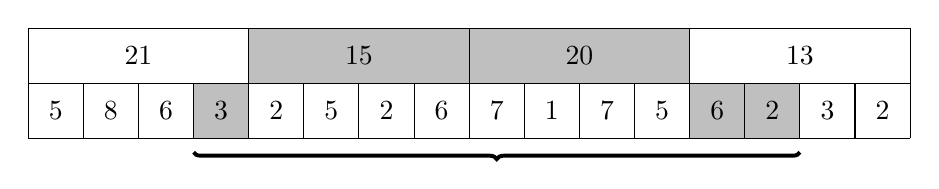
\begin{tikzpicture}[scale=0.7]
        \fill[color=lightgray] (3,0) rectangle (4,1);
        \fill[color=lightgray] (12,0) rectangle (13,1);
        \fill[color=lightgray] (13,0) rectangle (14,1);
        \draw (0,0) grid (16,1);

        \fill[color=lightgray] (4,1) rectangle (8,2);
        \fill[color=lightgray] (8,1) rectangle (12,2);
        \draw (0,1) rectangle (4,2);
        \draw (4,1) rectangle (8,2);
        \draw (8,1) rectangle (12,2);
        \draw (12,1) rectangle (16,2);

        \node at (0.5, 0.5) {5};
        \node at (1.5, 0.5) {8};
        \node at (2.5, 0.5) {6};
        \node at (3.5, 0.5) {3};
        \node at (4.5, 0.5) {2};
        \node at (5.5, 0.5) {5};
        \node at (6.5, 0.5) {2};
        \node at (7.5, 0.5) {6};
        \node at (8.5, 0.5) {7};
        \node at (9.5, 0.5) {1};
        \node at (10.5, 0.5) {7};
        \node at (11.5, 0.5) {5};
        \node at (12.5, 0.5) {6};
        \node at (13.5, 0.5) {2};
        \node at (14.5, 0.5) {3};
        \node at (15.5, 0.5) {2};

        \node at (2, 1.5) {21};
        \node at (6, 1.5) {15};
        \node at (10, 1.5) {20};
        \node at (14, 1.5) {13};

        \draw [decoration={brace}, decorate, line width=0.5mm] (14,-0.25) -- (3,-0.25);

    \end{tikzpicture}
\end{center}

Ya que el número de elementos individuales es como mucho $O(\sqrt n)$ y
el número de bloques también es $O(\sqrt n)$, la consulta de suma tarda
$O(\sqrt n)$. El propósito del tamaño de bloque $\sqrt n$ es que
\emph{equilibre} dos cosas: el arreglo se divide en $\sqrt n$ bloques,
cada uno de los cuales contiene $\sqrt n$ elementos.

En la práctica, no es necesario usar el valor exacto de $\sqrt n$ como
parámetro, y podemos usar los parámetros $k$ y $n/k$ donde $k$ es diferente de
$\sqrt n$. El parámetro óptimo depende del problema y la entrada. Por
ejemplo, si un algoritmo recorre los bloques a menudo pero raramente
inspecciona elementos individuales dentro de los bloques, puede ser una
buena idea dividir el arreglo en $k < \sqrt n$ bloques, cada uno de los
cuales contiene $n/k > \sqrt n$ elementos.

\section{Combinar algoritmos}

En esta sección veremos dos algoritmos de raíz cuadrada que se basan en
combinar dos algoritmos en uno. En ambos casos, podríamos usar alguno
de los algoritmos individualmente y resolver el problema en tiempo $O(n^2)$,
pero al combinar los algoritmos la complejidad se vuelve $O(n \sqrt n)$.

\subsubsection{Procesamiento por casos}

Supongamos que recibimos una grilla bidimensional que contiene $n$ celdas.
Cada celda es asignada una letra, y nuestra tarea es encontrar dos celdas
con la misma letra cuya distancia sea mínima, donde la distancia entre las
celdas $(x_1,y_1)$ y $(x_2,y_2)$ es $|x_1-x_2|+|y_1-y_2|$. Por ejemplo,
considera la siguiente grilla:

\begin{center}
    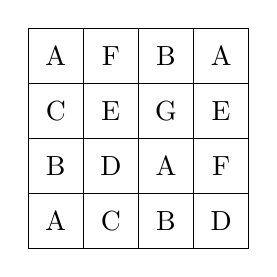
\begin{tikzpicture}[scale=0.7]
        \node at (0.5,0.5) {A};
        \node at (0.5,1.5) {B};
        \node at (0.5,2.5) {C};
        \node at (0.5,3.5) {A};
        \node at (1.5,0.5) {C};
        \node at (1.5,1.5) {D};
        \node at (1.5,2.5) {E};
        \node at (1.5,3.5) {F};
        \node at (2.5,0.5) {B};
        \node at (2.5,1.5) {A};
        \node at (2.5,2.5) {G};
        \node at (2.5,3.5) {B};
        \node at (3.5,0.5) {D};
        \node at (3.5,1.5) {F};
        \node at (3.5,2.5) {E};
        \node at (3.5,3.5) {A};
        \draw (0,0) grid (4,4);
    \end{tikzpicture}
\end{center}
En este caso, la distancia mínima es 2, entre las dos letras `E'.

Podemos resolver el problema considerando cada letra separadamente.
Usando este método, el nuevo problema es calcular la distancia mínima
entre dos celdas con una letra \emph{fija} $c$. Nos centraremos en dos
algoritmos para lograr esto:

\emph{Algoritmo 1}: Recorrer todos los pares de celdas con la letra $c$,
y calcular la mínima distancia entre estos. Esto tardará $O(k^2)$ donde
$k$ es el número de celdas con la letra $c$.

\emph{Algoritmo 2}: Realizar una búsqueda en profundidad que
simultáneamente comienza en cada celda con la letra $c$. La distancia
mínima entre dos celdas con la letra $c$ será calculada en $O(n)$.

Una manera de resolver el problema es elegir uno de los algoritmos y
usarlo para todas las letras. Si usamos el Algoritmo 1, el tiempo de
ejecución es $O(n^2)$, porque todas las celdas podrían contener la misma
letra, y en este caso $k=n$. Igualmente, con el Algoritmo 2 la complejidad
es $O(n^2)$, porque todas las celdas pueden tener letras distintas y en
este caso se requieren $n$ búsquedas.

De todas formas, podemos \emph{combinar} los dos algoritmos y usar uno
diferente para cada letra dependiendo de cuántas veces aparece cada letra
en nuestra grilla. Asume que una letra $c$ aparece $k$ veces. Si
$k \le \sqrt n$, usamos el Algoritmo 1, y si $k > \sqrt n$, usamos el
Algoritmo 2. Resulta que si hacemos esto, la complejidad temporal total
del algoritmo se vuelve $O(n \sqrt n)$.

Primero, supongamos que usamos el Algoritmo 1 para una letra $c$. Ya que
$c$ aparece como mucho $\sqrt n$ veces en la grilla, comparamos las celdas
$c$ $O(\sqrt n)$ veces entre ellas. Por lo tanto, el tiempo
utilizado para procesar todas estas celdas es $O(n \sqrt n)$. Ahora,
supongamos que usamos el Algoritmo 2 para una letra $c$. Hay como mucho
$\sqrt n$ letras tales, por lo que procesarlas también tarda $O(n \sqrt n)$.

\subsubsection{Procesamiento en lotes}

Nuestro siguiente problema también lidia con una grilla bidimensional
que contiene $n$ celdas. Inicialmente, todas menos una celda son blancas.
Realizamos $n-1$ operaciones, cada una de las cuales calcula la
distancia mínima desde una celda blanca dada a cualquier celda negra,
y luego pinta la celda blanca de negro.

Por ejemplo, considera la siguiente operación:

\begin{center}
    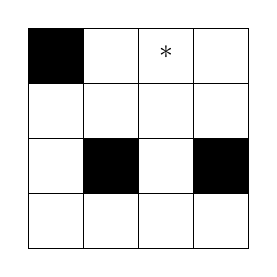
\begin{tikzpicture}[scale=0.7]
        \fill[color=black] (1,1) rectangle (2,2);
        \fill[color=black] (3,1) rectangle (4,2);
        \fill[color=black] (0,3) rectangle (1,4);
        \node at (2.5,3.5) {*};
        \draw (0,0) grid (4,4);
    \end{tikzpicture}
\end{center}

Primero, calculamos la distancia mínima de la celda blanca marcada con *
a alguna celda negra. La distancia mínima es 2, porque podemos movernos dos
pasos a la izquierda hacia una celda negra. Luego, pintamos la celda
de negro:

\begin{center}
    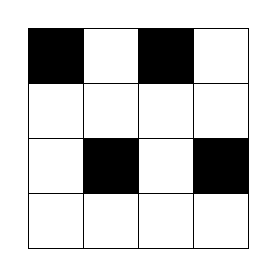
\begin{tikzpicture}[scale=0.7]
        \fill[color=black] (1,1) rectangle (2,2);
        \fill[color=black] (3,1) rectangle (4,2);
        \fill[color=black] (0,3) rectangle (1,4);
        \fill[color=black] (2,3) rectangle (3,4);
        \draw (0,0) grid (4,4);
    \end{tikzpicture}
\end{center}

Considera los dos siguientes algoritmos:

\emph{Algoritmo 1}: Usar búsqueda en anchura para encontrar la celda negra
más cercana de cada celda blanca. Esto tarda $O(n)$, y luego de la búsqueda
podemos encontrar la distancia mínima de cualquier blanca a cualquier negra
en $O(1)$.

\emph{Algoritmo 2}: Mantener una lista de celdas que se hayan pintado de
negro, recorrer esta lista en cada operación y luego añadir una nueva
celda a la lista. Una operación tarda $O(k)$ donde $k$ es la longitud
de la lista.

Combinamos los dos algoritmos de arriba dividiendo las operaciones en
$O(\sqrt n)$ \emph{lotes}, cada uno de los cuales consiste de $O(\sqrt n)$
operaciones. Al principio de cada lote, ejecutamos el Algoritmo 1. Luego,
usamos el Algoritmo 2 para procesar las operaciones en el lote. Vaciamos
la lista del Algoritmo 2 entre lotes. En cada operación, la distancia
mínima a alguna celda negra es aquella calculada por el Algoritmo 1
o aquella calculada por el Algoritmo 2.

El algoritmo resultante tiene una complejidad de $O(n \sqrt n)$. Primero,
el Algoritmo 1 se ejecuta $O(\sqrt n)$ veces, y cada búsqueda funciona en
$O(n)$. Segundo, cuando usamos el Algoritmo 2 en un lote, la lista contiene
$O(\sqrt n)$ celdas (porque vaciamos la lista entre lotes) y cada operación
tarda $O(\sqrt n)$.

\section{Particiones de enteros}

Algunos algoritmos de raíz cuadrada se basan en lo siguiente:
si un entero positivo $n$ está representado como una suma de enteros
positivos, tal suma contiene a lo sumo $O(\sqrt n)$ números
\emph{distintos}. La razón es que para construir una suma con la mayor
cantidad de números distintos posibles, debemos elegir números
\emph{pequeños}. Si elegimos los números $1,2,\ldots,k$, la suma resultante
es \[\frac{k(k+1)}{2}.\] Por ende, la máxima cantidad de números distintos
es $k = O(\sqrt n)$. Veremos dos problemas que pueden resolverse
eficientemente usando esta observación.

\subsubsection{Mochila}

Supongamos que recibimos una lista de pesos enteros cuya suma es $n$.
Nuestra tarea es encontrar todas las sumas que se pueden formar con un
subconjunto de los pesos. Por ejemplo, si los pesos son $\{1,3,3\}$,
las sumas posibles son:

\begin{itemize}[noitemsep]
    \item $0$ (vacía)
    \item $1$
    \item $3$
    \item $1+3=4$
    \item $3+3=6$
    \item $1+3+3=7$
\end{itemize}

Utilizando el método de la mochila (ver Capítulo 7.4),
el problema puede resolverse de la siguiente forma: definimos una función
$\texttt{posible}(x,k)$ cuyo valor es 1 si la suma $x$ puede formarse
usando los primeros $k$ pesos, y de lo contrario es 0. Ya que la suma de
los pesos es $n$, hay como máximo $n$ pesos y todos los valores de la
función pueden calcularse en $O(n^2)$ utilizando programación dinámica.

No obstante, podemos optimizar el algoritmo si usamos el hecho de que hay
como máximo $O(\sqrt n)$ pesos \emph{distintos}. Por esto, podemos procesar
los pesos en grupos que consisten de pesos similares. Podemos procesar
cada grupo en $O(n)$, lo que resulta en un algoritmo de $O(n \sqrt n)$.

La idea es usar un arreglo que registre las sumas de pesos que pueden
formarse usando los grupos procesados hasta ahora. El arreglo contiene
$n$ elementos: el elemento $k$ es 1 si la suma $k$ puede formarse y 0
de lo contrario. Para procesar un grupo de pesos, recorremos el arreglo
de izquierda a derecha y registramos las nuevas sumas que pueden formarse
usando este grupo y los grupos previos.

\subsubsection{Construcción de cadenas}

Dada una cadena \texttt{s} de longitud $n$ y un conjunto de cadenas $D$
cuya longitud total sea $m$, debemos contar el número de
formas en que \texttt{s} puede formarse como una concatenación de
cadenas en $D$. Por ejemplo, si $\texttt{s}=\texttt{ABAB}$ y
$D=\{\texttt{A},\texttt{B},\texttt{AB}\}$, existen 4:

\begin{itemize}[noitemsep]
    \item $\texttt{A}+\texttt{B}+\texttt{A}+\texttt{B}$
    \item $\texttt{AB}+\texttt{A}+\texttt{B}$
    \item $\texttt{A}+\texttt{B}+\texttt{AB}$
    \item $\texttt{AB}+\texttt{AB}$
\end{itemize}

Podemos resolver el problema usando programación dinámica: Definamos
$\texttt{conteo}(k)$ como el número de maneras de construir el prefijo
$\texttt{s}[0 \ldots k]$ usando las cadenas en $D$. Ahora
$\texttt{conteo}(n-1)$ nos da la respuesta al problema, y podemos resolverlo
en $O(n^2)$ usando un trie.

Sin embargo, podemos resolver el problema más eficientemente utilizando
el hashing de cadenas y el hecho de que hay a lo sumo $O(\sqrt m)$ longitudes
de cadenas distintas en $D$. Primero, construimos un conjunto $H$ que
contiene todos los valores de hash de las cadenas en $D$.
Luego, al calcular un valor de $\texttt{conteo}(k)$, recorremos todos los
valores de $p$ tal que haya una cadena de longitud $p$ en $D$, calculamos
el valor de hash de $\texttt{s}[k-p+1 \ldots k]$ y revisamos si pertenece
a $H$. Debido a que hay, a lo sumo, $O(\sqrt m)$ longitudes de cadena
distintas, esto resulta en un algoritmo cuya complejidad temporal es
$O(n \sqrt m)$.

\section{Algoritmo de Mo}

\index{algoritmo de!Mo}

El \key{algoritmo de Mo}\footnote{Según \cite{cod15}, este algoritmo lleva
    el nombre de Mo Tao, un programador competitivo chino, pero la técnica
    ha aparecido antes en la literatura \cite{ken06}.} puede utilizarse en
muchos problemas que requieren procesar consultas en rangos sobre arreglos
\emph{estáticos}, donde los valores no cambian entre consultas.
En cada consulta recibimos un rango $[a,b]$ y debemos calcular un valor en
base a los elementos del arreglo entre las posiciones $a$ y $b$. Ya que el
arreglo es estático, las consultas pueden procesare en cualquier orden, y
el algoritmo de Mo las procesa en un orden especial que lo hace eficiente.

El algoritmo de Mo mantiene un \emph{rango activo} en el arreglo, y la
respuesta a una consulta sobre el rango activo se conoce en cada momento.
El algoritmo procesa las consultas una tras otra, y siempre mueve los
extremos del rango activo insertando y removiendo elementos. La complejidad
temporal del algoritmo es $O(n \sqrt n f(n))$ donde $n$ es la longitud del
arreglo, se hacen $n$ consultas, y cada inserción y remoción de un elemento
tarda $O(f(n))$.

El truco del algoritmo de Mo es el orden en que se procesan las consultas:
el arreglo se divide en bloques de $k=O(\sqrt n)$ elementos, y una consulta
$[a_1,b_1]$ se procesa antes que otra $[a_2,b_2]$ si
\begin{itemize}
    \item $\lfloor a_1/k \rfloor < \lfloor a_2/k \rfloor$ \emph{o}
    \item $\lfloor a_1/k \rfloor = \lfloor a_2/k \rfloor$ y $b_1 < b_2$.
\end{itemize}

Por ende, todas las consultas cuyos extremos izquierdos estén en cierto
bloque se procesan una tras otra según sus extremos derechos. Usando este
orden, el algoritmo solo realiza $O(n \sqrt n)$ operaciones, porque el
extremo izquierdo se mueve $O(\sqrt n)$ pasos $O(n)$ veces, y el extremo
derecho se mueve $O(n)$ pasos $O(\sqrt n)$ veces. Entonces, ambos extremos
se mueven un total de $O(n \sqrt n)$ pasos durante el algoritmo.

\subsubsection*{Ejemplo}

Como ejemplo, veamos un problema donde recibimos un conjunto de consultas,
cada una correspondiente a un rango en el arreglo, y nuestra tarea es
calcular, para cada una, el número de elementos \emph{distintos} en el rango.

En el algoritmo de Mo, las consultas siempre se ordenan de la misma manera,
pero depende del problema cómo se mantiene la respuesta a la consulta.
En este problema, podemos mantener un arreglo \texttt{veces}
donde $\texttt{veces}[x]$ indica el número de veces que un elemento
$x$ ocurre en el rango activo.

Cuando nos movemos de una consulta a otra, el rango activo cambia. Por
ejemplo, si el rango actual es
\begin{center}
    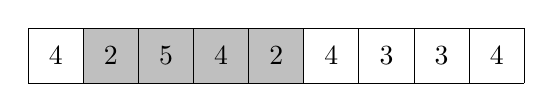
\begin{tikzpicture}[scale=0.7]
        \fill[color=lightgray] (1,0) rectangle (5,1);
        \draw (0,0) grid (9,1);
        \node at (0.5, 0.5) {4};
        \node at (1.5, 0.5) {2};
        \node at (2.5, 0.5) {5};
        \node at (3.5, 0.5) {4};
        \node at (4.5, 0.5) {2};
        \node at (5.5, 0.5) {4};
        \node at (6.5, 0.5) {3};
        \node at (7.5, 0.5) {3};
        \node at (8.5, 0.5) {4};
    \end{tikzpicture}
\end{center}
y el siguiente rango es
\begin{center}
    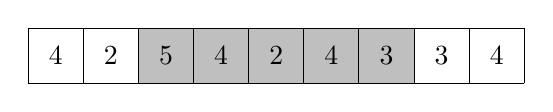
\begin{tikzpicture}[scale=0.7]
        \fill[color=lightgray] (2,0) rectangle (7,1);
        \draw (0,0) grid (9,1);
        \node at (0.5, 0.5) {4};
        \node at (1.5, 0.5) {2};
        \node at (2.5, 0.5) {5};
        \node at (3.5, 0.5) {4};
        \node at (4.5, 0.5) {2};
        \node at (5.5, 0.5) {4};
        \node at (6.5, 0.5) {3};
        \node at (7.5, 0.5) {3};
        \node at (8.5, 0.5) {4};
    \end{tikzpicture}
\end{center}
habrá tres pasos: el extremo izquierdo se mueve un paso a la derecha, y el
extremo derecho se mueve dos pasos a la derecha.

Luego de cada paso, el arreglo \texttt{veces} debe actualizarse. Tras
añadir un elemento $x$, aumentamos el valor de $\texttt{veces}[x]$ por 1,
y si ahora $\texttt{veces}[x]=1$, también aumentamos la respuesta
a la consulta por 1. Similarmente, luego de quitar un elemento $x$,
disminuimos el valor de $\texttt{veces}[x]$ por 1, y si
ahora $\texttt{veces}[x]=0$, también disminuimos la respuesta
a la consulta por 1.

En este problema, el tiempo necesario para realizar cada paso es $O(1)$,
así que la complejidad temporal total del algoritmo es $O(n \sqrt n)$.